\chapter{Virology}\label{ch:b3:virology}

There are some $10^{31}$ \omterm{def:b3:virology:virus}{virus} particles on Earth, ten for every cell,
and in the sea they kill a fifth of all bacteria every day. A \omterm{def:b3:virology:virus}{virus} is
not a cell: it has no metabolism, no ribosomes, no way to make anything
by itself. It is a genome --- as short as two genes, as long as two
thousand --- wrapped in a protein shell, which enters a cell and turns
the cell's machinery to making copies of itself. The influenza of 1918
killed fifty million people; smallpox, which killed three hundred
million in the twentieth century alone, was eradicated in 1980 by a
\omterm{def:b3:virology:drugs}{vaccine} first tried in 1796; and a coronavirus that crossed into humans
in 2019 had its genome sequenced within weeks, a \omterm{def:b3:virology:drugs}{vaccine} designed within
days of that, and drugs against its protease within two years. This
chapter treats what viruses are and how they are classified by the
chemistry of their genomes, how they multiply, the kinetics of an
infection inside one host --- which a pair of differential equations
describes well enough to have changed the treatment of AIDS --- their
evolution, and how they are fought.

\section{What a virus is}

\begin{definition}[Virus]\label{def:b3:virology:virus}
\index{virus}\index{capsid}\index{envelope}\index{virion}\index{Baltimore classification}
A \emph{virus} is an obligate intracellular parasite consisting of a
nucleic acid genome --- DNA or RNA, single- or double-stranded, linear
or circular, one molecule or several --- packaged in a protein
\emph{capsid}, and in many cases wrapped in an \emph{envelope} taken
from a host membrane and studded with viral glycoproteins. The complete
infectious particle is the \emph{virion}, \qtyrange{20}{300}{nm} across
for most (a few giant viruses reach a micrometre). Capsids are built
from many copies of one or a few proteins arranged with helical
symmetry (a rod, as in tobacco mosaic virus) or icosahedral symmetry (a
shell of $60T$ subunits, $T = 1, 3, 4, 7,\dots$). The \emph{Baltimore
classification} groups viruses by the route from genome to messenger
RNA: I, double-stranded DNA (herpes, pox, adenovirus, most phages); II,
single-stranded DNA (parvovirus); III, double-stranded RNA (rotavirus);
IV, positive-strand RNA, itself a messenger (polio, hepatitis C, the
coronaviruses); V, negative-strand RNA, complementary to messenger
(influenza, measles, rabies, Ebola); VI, RNA reverse-transcribed into
DNA (the retroviruses, HIV); VII, DNA replicated through an RNA
intermediate (hepatitis B). Every class but I must bring or encode an
enzyme the cell lacks --- an RNA-dependent RNA polymerase, a reverse
transcriptase --- and those enzymes are the targets of most \omterm{def:b3:virology:drugs}{antiviral
drugs}.
\end{definition}

\begin{proof}[Evidence]
Ivanovsky (1892) and Beijerinck (1898) showed that the mosaic disease of
tobacco was transmitted by sap passed through filters that retained all
bacteria --- a \emph{contagium vivum fluidum}, a living infectious
fluid. Stanley (1935) crystallised the agent, tobacco mosaic \omterm{def:b3:virology:virus}{virus}, and
showed it to be protein with (as Bawden and Pirie found) \qty{5}{\%}
RNA. Hershey and Chase (1952) labelled a bacteriophage's protein with
$^{35}$S and its DNA with $^{32}$P, let it infect \emph{E.~coli},
sheared off the empty coats in a blender, and found the $^{32}$P inside
the cells and the $^{35}$S outside: the DNA enters and the protein
stays behind, so the DNA carries the instructions. Fraenkel-Conrat
(1955) took tobacco mosaic \omterm{def:b3:virology:virus}{virus} apart into protein and RNA and
reassembled infectious particles from the RNA of one strain and the
protein of another; the progeny were of the RNA's strain.
\end{proof}

\begin{proposition}[Genetic economy: why capsids are symmetric]\label{prop:b3:virology:economy}
\index{genetic economy}
A \omterm{def:b3:virology:virus}{capsid} must enclose the genome that encodes it. A protein of mass
$m$ needs about $m/\qty{110}{Da}$ codons, that is $3m/110$ nucleotides,
a stretch of RNA weighing about $3m/110\times\qty{330}{Da} = 9m$: any
protein is encoded by a nucleic acid nine times its own mass. A shell
made of a \emph{single} protein molecule enclosing a genome would have
to enclose a genome nine times its own mass just to encode itself, and
a shell cannot hold nine times its own mass of nucleic acid at
biological density. The way out, seen by Crick and Watson (1956), is to
build the shell from many copies of one small protein: tobacco mosaic
\omterm{def:b3:virology:virus}{virus} encodes a \qty{17.5}{kDa} coat protein in \qty{480}{nt} of its
\qty{6400}{nt} genome and uses $2130$ copies of it. Identical subunits
that pack identically must be arranged symmetrically, so viral \omterm{def:b3:virology:virus}{capsids}
are helices or icosahedra, and the same economy gives them the
capacity to self-assemble, since each subunit needs only to recognise
its neighbours.
\end{proposition}
\begin{proof}
The mass ratio follows from a codon being three nucleotides of about
\qty{330}{Da} each and a residue about \qty{110}{Da}: $3\times 330/110 =
9$. A \omterm{def:b3:virology:virus}{capsid} of one \qty{40}{MDa} protein would enclose \qty{360}{MDa}
of nucleic acid, a sphere of radius about \qty{50}{nm} at nucleic-acid
density, whereas the protein itself would make a shell of about
\qty{2}{nm} thickness and the same radius --- geometrically possible,
but a single polypeptide of $360\,000$ residues that folds correctly is
not, and one mutation would destroy it. With $n$ identical subunits the
coding cost falls by $n$ while the enclosed volume is unchanged.
\end{proof}

\begin{omfigure}
\begin{tikzpicture}[every node/.style={font=\scriptsize}, >=stealth]
  \node[draw, thick, rounded corners, fill=omMeth!30, minimum width=2.4cm] (mrna) at (0,0) {mRNA $\to$ protein};
  \node[draw, thick, rounded corners, fill=omDef!20, align=center] (I) at (-5.8,3.6) {I: dsDNA\\herpes, pox, phage T4};
  \node[draw, thick, rounded corners, fill=omDef!20, align=center] (II) at (-2.0,3.6) {II: ssDNA\\parvovirus};
  \node[draw, thick, rounded corners, fill=omThm!20, align=center] (III) at (2.0,3.6) {III: dsRNA\\rotavirus};
  \node[draw, thick, rounded corners, fill=omThm!20, align=center] (IV) at (5.8,3.6) {IV: (+)RNA\\polio, hepatitis C,\\coronaviruses};
  \node[draw, thick, rounded corners, fill=omThm!20, align=center] (V) at (-5.6,-3.4) {V: ($-$)RNA\\influenza, measles,\\rabies, Ebola};
  \node[draw, thick, rounded corners, fill=omProp!30, align=center] (VI) at (0,-3.4) {VI: RNA $\to$ DNA\\retroviruses (HIV)};
  \node[draw, thick, rounded corners, fill=omProp!30, align=center] (VII) at (5.6,-3.4) {VII: DNA via RNA\\hepatitis B};
  \node[below, font=\tiny, align=center, gray!50!black] at (-5.8,2.9) {host RNA polymerase};
  \node[below, font=\tiny, align=center, gray!50!black] at (-2.0,3.05) {second strand made,\\then transcription};
  \node[below, font=\tiny, align=center, gray!50!black] at (2.0,3.05) {viral RNA polymerase\\in the particle};
  \node[below, font=\tiny, align=center, gray!50!black] at (5.8,2.75) {the genome is the mRNA};
  \node[above, font=\tiny, align=center, gray!50!black] at (-5.6,-2.55) {viral polymerase copies it};
  \node[above, font=\tiny, align=center, gray!50!black] at (0,-2.85) {reverse transcriptase, integration,\\then host polymerase};
  \node[above, font=\tiny, align=center, gray!50!black] at (5.6,-2.85) {transcription of the DNA};
  \foreach \c in {I,II,III,IV,V,VI,VII} \draw[->, thick] (\c) -- (mrna);
\end{tikzpicture}

{\small The seven Baltimore classes, sorted by the route from genome to
messenger RNA. Every class except I needs an enzyme the host cell does
not provide --- the natural target of an \omterm{def:b3:virology:drugs}{antiviral drug}.}
\end{omfigure}

\begin{omfigure}
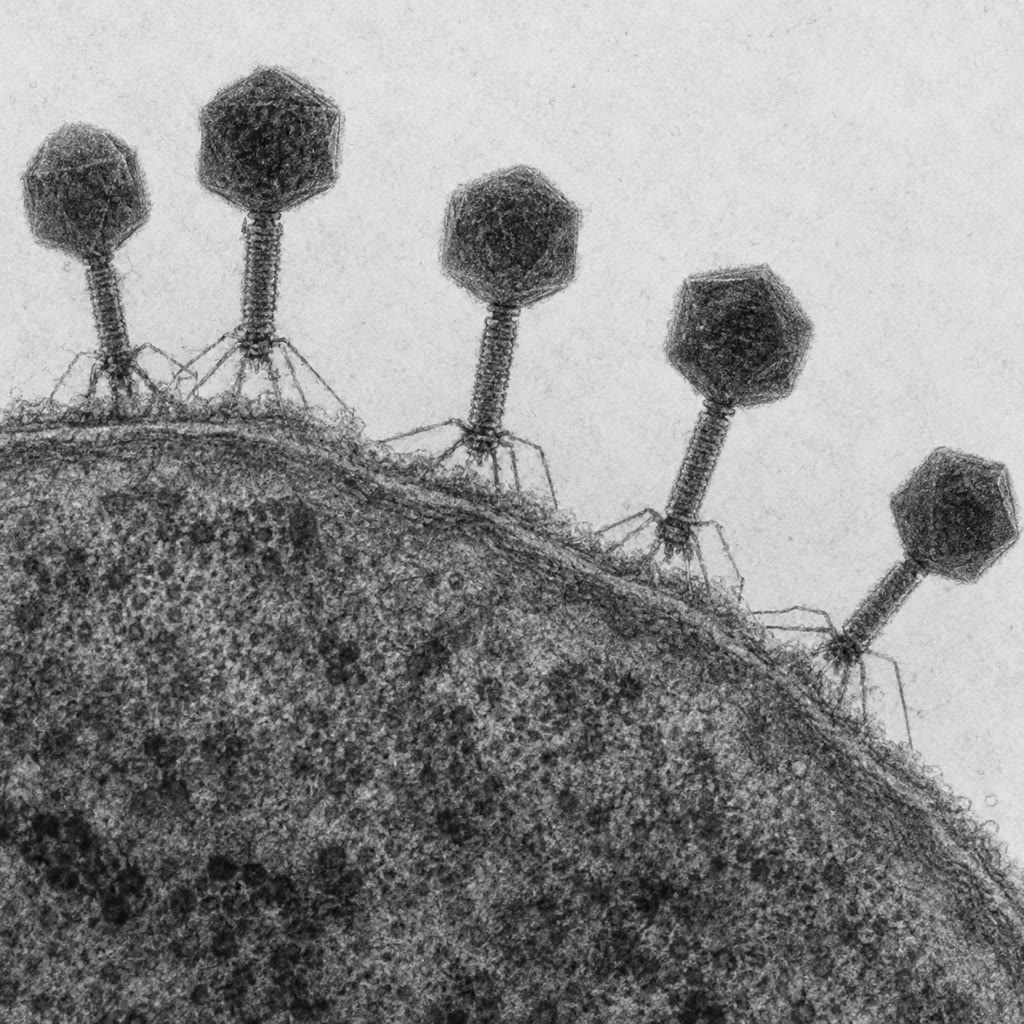
\includegraphics[width=0.36\linewidth]{images/book5/ai/b5-13-phage-tem.jpg}\hspace{0.04\linewidth}
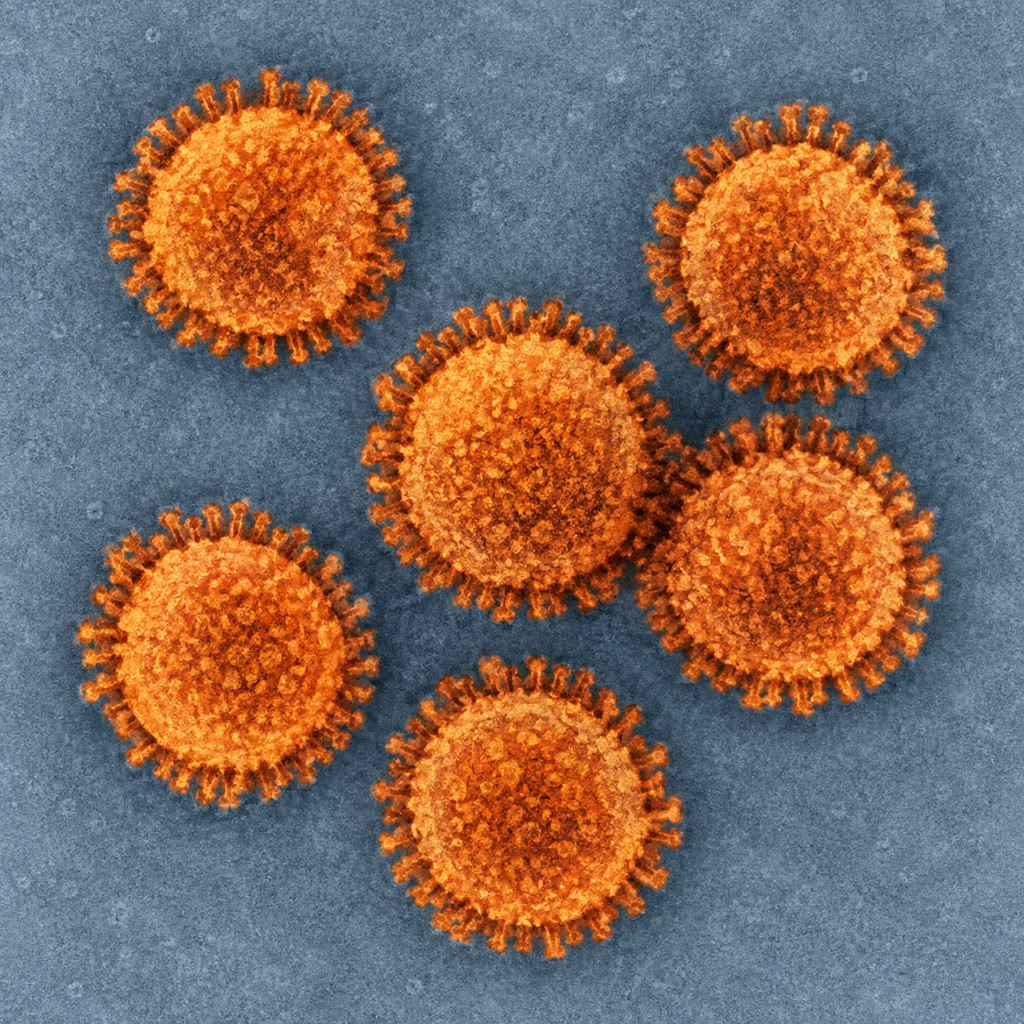
\includegraphics[width=0.36\linewidth]{images/book5/ai/b5-13-influenza-virions.jpg}

{\small Left: bacteriophages attached by their tail fibres to a
bacterium, each head an icosahedral \omterm{def:b3:virology:virus}{capsid} of DNA. Right: influenza
\omterm{def:b3:virology:virus}{virions}, enveloped, their surface a fringe of haemagglutinin and
neuraminidase spikes.}
\end{omfigure}

\section{How a virus multiplies}

\begin{definition}[The replication cycle]\label{def:b3:virology:cycle}
\index{viral replication cycle}\index{receptor!viral}\index{lysogeny}\index{latency}
Every \omterm{def:b3:virology:virus}{virus} passes through the same stages. \emph{Attachment} to a
specific host receptor --- CD4 and a chemokine receptor for HIV, ACE2
for the SARS coronaviruses, sialic acid for influenza, a
\omterm{def:b3:bacteriology:envelope}{lipopolysaccharide} or a porin for a phage --- which decides which
species and which cells the \omterm{def:b3:virology:virus}{virus} can infect (its \emph{tropism}).
\emph{Entry}: fusion of the \omterm{def:b3:virology:virus}{envelope} with the plasma membrane, or
endocytosis followed by fusion from within the acid \omterm{def:b3:membrane-traffic:endocytosis}{endosome}, or, for
a phage, injection of the genome through the wall. \emph{Uncoating},
\emph{expression} of the viral genes by the class-specific route, and
\emph{replication} of the genome, often in a factory the \omterm{def:b3:virology:virus}{virus} builds
in the cytoplasm or nucleus. \emph{Assembly} of new \omterm{def:b3:virology:virus}{capsids} around new
genomes, driven by the self-assembly of the symmetric subunits, and
\emph{release}: by lysis of the cell, or by budding through a membrane,
which supplies the \omterm{def:b3:virology:virus}{envelope}. Some viruses can instead insert their
genome into the host's and wait: the \emph{lysogeny} of phage $\lambda$,
whose repressor keeps it silent until the host is damaged; the
\emph{latency} of herpesviruses in neurons for a lifetime and of HIV as
a provirus in resting T~cells, from which it is not removed by any
drug that acts on replication.
\end{definition}

\begin{omfigure}
\begin{tikzpicture}[every node/.style={font=\scriptsize}, >=stealth]
  % cell
  \draw[very thick, omDef, fill=omDef!6] (0,0) ellipse (5.6 and 3.2);
  \draw[thick, omDef!70, fill=omDef!20] (1.8,0) ellipse (1.6 and 1.1); \node at (1.8,0.75) {nucleus};
  % virion outside
  \draw[thick, omProp, fill=omProp!30] (-7.2,1.6) circle (0.35); \foreach \a in {0,45,...,315} \draw[omProp, thick] (-7.2,1.6) ++(\a:0.35) -- ++(\a:0.15);
  \node[above] at (-7.2,2.1) {virion};
  \draw[->, thick] (-6.8,1.4) -- (-5.7,0.9); \node[below, align=center] at (-6.6,1.0) {1. attach to\\receptor};
  % entry
  \draw[thick, omProp] (-5.4,0.7) arc[start angle=140, end angle=40, radius=0.5];
  \node[below, align=center] at (-3.9,-0.2) {2. fuse or endocytose;\\3. uncoat};
  % genome path
  \draw[omThm, very thick] (-3.4,0.2) .. controls (-2.6,0.6) .. (-1.8,0.4);
  \draw[->, thick] (-1.6,0.4) -- (-0.4,0.4);
  \node[above, align=center] at (-1.0,0.55) {4. express genes,\\replicate genome};
  \draw[omThm, very thick] (-1.0,-0.5) -- (0.4,-0.5); \draw[omThm, very thick] (-1.0,-0.75) -- (0.4,-0.75); \draw[omThm, very thick] (-1.0,-1.0) -- (0.4,-1.0);
  % assembly
  \foreach \p in {(1.2,-1.6),(1.9,-1.9),(2.6,-1.5)} { \draw[thick, omProp, fill=omProp!30] \p circle (0.25); }
  \node[below, align=center] at (1.9,-2.2) {5. assemble capsids\\around genomes};
  % budding
  \draw[thick, omProp, fill=omProp!30] (4.9,-1.7) circle (0.32); \draw[->, thick] (5.3,-1.75) -- (6.4,-2.0);
  \draw[thick, omProp, fill=omProp!30] (7.0,-2.2) circle (0.35); \foreach \a in {0,45,...,315} \draw[omProp, thick] (7.0,-2.2) ++(\a:0.35) -- ++(\a:0.15);
  \node[below, align=center] at (6.4,-2.6) {6. bud through the membrane\\(envelope) or lyse the cell};
  % latency
  \draw[->, thick, dashed, omMeth!70!black] (-0.2,0.2) -- (0.9,0.2); \node[below, omMeth!70!black, align=center, font=\tiny] at (2.0,-0.05) {retroviruses: integrate\\as a provirus; latency};
\end{tikzpicture}

{\small The replication cycle of an enveloped \omterm{def:b3:virology:virus}{virus}: attachment to a
receptor, entry and uncoating, expression and replication in the host's
machinery, assembly, and release by budding --- or, for a retrovirus,
integration into the host genome and silence.}
\end{omfigure}

\begin{method}[Counting infectious particles: the plaque assay]\label{met:b3:virology:plaque}
\index{plaque assay}\index{titre}
To measure a \omterm{def:b3:virology:virus}{virus} stock: (1) dilute it in tenfold steps; (2) mix each
dilution with an excess of host cells --- bacteria in soft agar for a
phage, a monolayer of cultured cells for an animal \omterm{def:b3:virology:virus}{virus}; (3) incubate:
each infectious particle infects one cell, the progeny infect the
neighbours, and after a day or two a clear hole, a \emph{plaque},
marks the spot; (4) count the plaques on a plate with \numrange{30}{300}
and multiply by the dilution: the \emph{titre} in plaque-forming units
(PFU) per millilitre. Since each plaque is a clone of one particle,
picking it yields a pure isolate. The ratio of physical particles
(counted by electron microscopy or PCR) to plaque-forming units is
usually far above one --- ten to a thousand for many animal viruses ---
since most particles are defective or fail to infect.
\end{method}

\begin{omfigure}
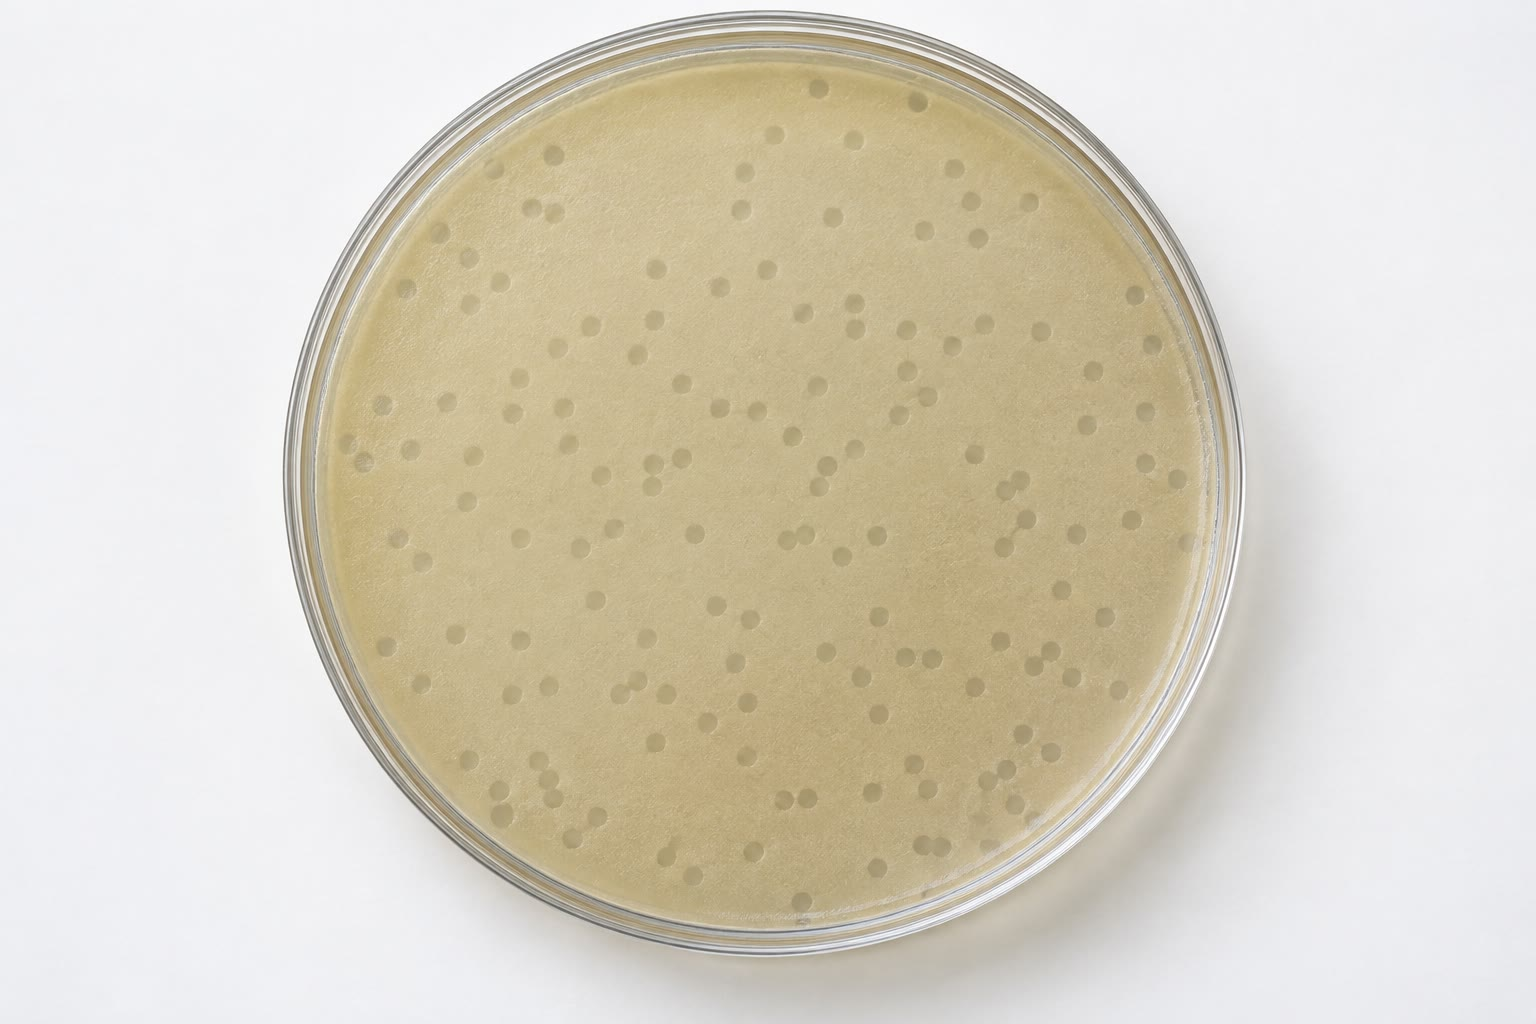
\includegraphics[width=0.46\linewidth]{images/book5/ai/b5-13-plaque-assay.jpg}\hspace{0.04\linewidth}
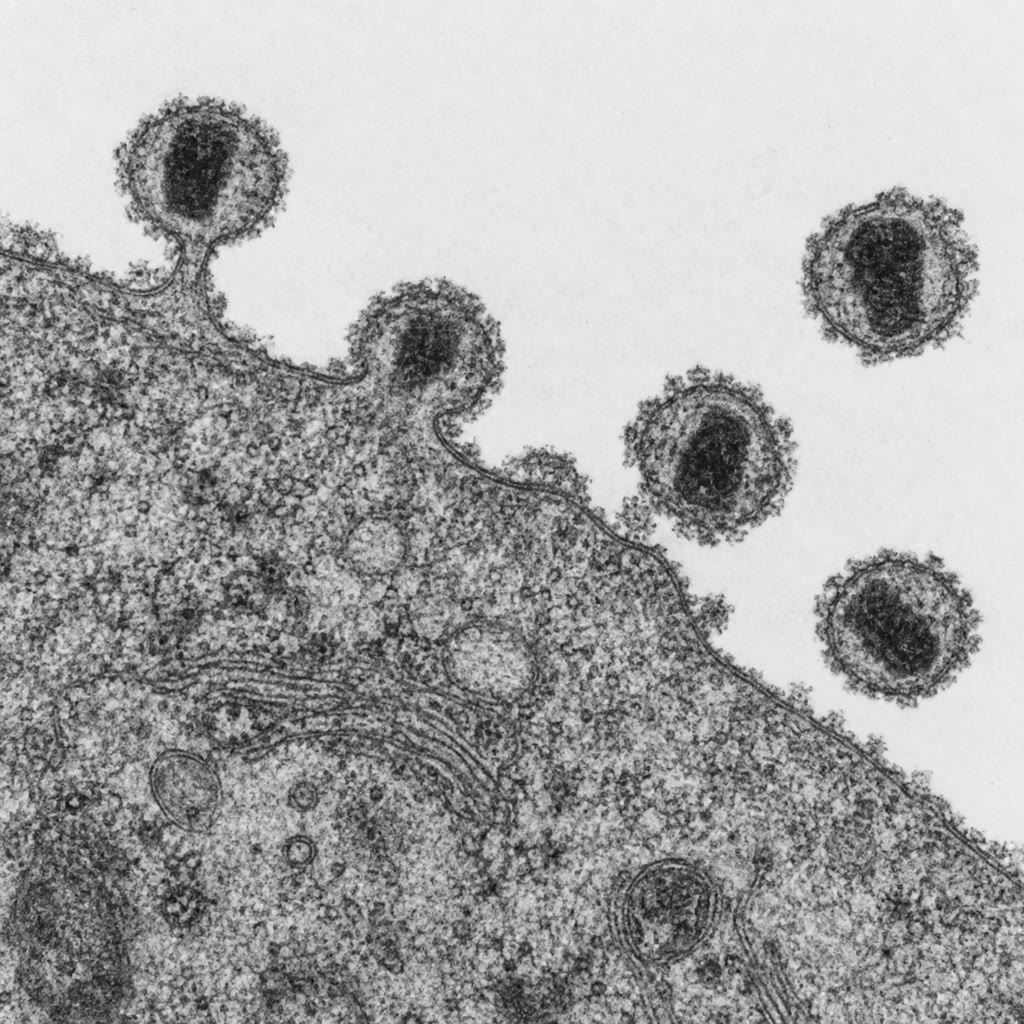
\includegraphics[width=0.36\linewidth]{images/book5/ai/b5-13-hiv-budding.jpg}

{\small Left: plaques in a bacterial lawn, each a clear zone where the
progeny of one phage have lysed the cells around it. Right: HIV
particles budding from a T~lymphocyte, taking their \omterm{def:b3:virology:virus}{envelope} from the
cell's membrane.}
\end{omfigure}

\begin{theorem}[Infection dynamics within a host]\label{thm:b3:virology:dynamics}
\index{basic reproduction number!within-host}\index{viral load}\index{viral dynamics}
Let $T$ be the density of susceptible target cells, $I$ of infected
cells and $V$ of free \omterm{def:b3:virology:virus}{virions}. \omterm{def:b3:virology:virus}{Virions} infect targets at rate $\beta TV$,
infected cells produce \omterm{def:b3:virology:virus}{virions} at rate $p$ each and die at rate
$\delta$, and free \omterm{def:b3:virology:virus}{virions} are cleared at rate $c$:
\[
\frac{\mathrm{d}I}{\mathrm{d}t} = \beta TV - \delta I, \qquad
\frac{\mathrm{d}V}{\mathrm{d}t} = pI - cV .
\]
With $T$ held constant, the infection grows if the \emph{basic
reproduction number} $R_{0} = \beta Tp/(c\delta)$ exceeds $1$, and at
steady state $V^{*} = p I^{*}/c$ with production balancing clearance.
If a drug stops all new infections at $t = 0$ ($\beta \to 0$), the
\omterm{def:b3:virology:virus}{virions} decay at first at the clearance rate $c$, then, once the free
\omterm{def:b3:virology:virus}{virus} has fallen to the level the remaining infected cells maintain, at
the death rate $\delta$ of those cells:
\[
V(t) \approx V_{0}\,\frac{c\,e^{-\delta t} - \delta\,e^{-ct}}{c - \delta}
\;\longrightarrow\; V_{0}\,\frac{c}{c-\delta}\,e^{-\delta t}
\quad (t \gg 1/c).
\]
The two slopes of the \omterm{thm:b3:virology:dynamics}{viral load} after treatment measure $c$ and
$\delta$, and $pI^{*} = cV^{*}$ gives the daily production of \omterm{def:b3:virology:virus}{virions}
before treatment.
\end{theorem}
\begin{proof}
An infected cell lives on average $1/\delta$ and makes $p/\delta$
\omterm{def:b3:virology:virus}{virions}; each \omterm{def:b3:virology:virus}{virion} lives $1/c$ and infects $\beta T/c$ cells in that
time; the product is the number of infected cells one infected cell
gives rise to, $R_{0}$. At steady state $\mathrm{d}V/\mathrm{d}t = 0$
gives $V^{*} = pI^{*}/c$. After treatment $\mathrm{d}I/\mathrm{d}t =
-\delta I$, so $I = I_{0}e^{-\delta t}$, and $\mathrm{d}V/\mathrm{d}t =
pI_{0}e^{-\delta t} - cV$ is a linear equation whose solution with
$V(0) = V_{0} = pI_{0}/c$ is the expression given (check: at $t = 0$ it
equals $V_{0}$, and it satisfies the equation term by term). For $t
\gg 1/c$ the $e^{-ct}$ term is gone and $V$ follows the infected cells
with slope $-\delta$; for $t \ll 1/\delta$ and $c \gg \delta$ the early
slope is $-c$.
\end{proof}

\begin{example}[HIV before and after the equations]\label{ex:b3:virology:hiv}
Until 1995 the years of clinical \omterm{def:b3:virology:cycle}{latency} of HIV infection --- a stable
\omterm{thm:b3:virology:dynamics}{viral load} of $10^{4}$--$10^{6}$ copies per millilitre and a slow fall of
T~cells --- were read as a quiescent \omterm{def:b3:virology:virus}{virus}. Ho, Perelson and colleagues
gave patients a \omterm{def:b3:virology:drugs}{protease inhibitor} and fitted the decline of the \omterm{thm:b3:virology:dynamics}{viral
load} to the theorem: the fast phase gave $c \approx \qty{3}{d^{-1}}$
(a \omterm{def:b3:virology:virus}{virion} half-life of about six hours), the slow phase $\delta \approx
\qty{0.5}{d^{-1}}$ (an infected cell lives about a day and a half). A
steady load of $10^{5}$ per millilitre in \qty{15}{L} of body fluid,
cleared at $c$, therefore requires the production of about $10^{10}$
\omterm{def:b3:virology:virus}{virions} a day, every day, for years: the ``latent'' period is a
furious steady state of infection and death, with the T~cell pool
replaced daily until it fails. The mutation arithmetic of the next
section then follows at once, and with it the reason single drugs
failed and three did not.
\end{example}

\begin{omfigure}
\begin{tikzpicture}
\begin{axis}[
  width=0.7\linewidth, height=5.8cm,
  axis x line=bottom, axis y line=left,
  xmin=0, xmax=14, ymin=10, ymax=2e5, ymode=log,
  xlabel={days after starting therapy}, ylabel={virions per mL},
  xlabel style={font=\small, at={(axis description cs:0.5,-0.12)}, anchor=north}, ylabel style={font=\small},
  tick label style={font=\small}, xtick={0,2,4,6,8,10,12,14},
  clip=false,
]
\addplot[very thick, omDef, domain=0:14, samples=100] {1e5*(3*exp(-0.5*x) - 0.5*exp(-3*x))/2.5};
\addplot[dashed, omThm, domain=0:1.6, samples=2] {1e5*exp(-3*x)};
\addplot[dashed, omMeth!70!black, domain=1.5:14, samples=2] {1e5*1.2*exp(-0.5*x)};
\node[font=\scriptsize, omThm, anchor=west] at (axis cs:1.8,600) {free virions cleared: slope $-c$, half-life \qty{6}{h}};
\node[font=\scriptsize, omMeth!70!black, anchor=south west] at (axis cs:5.5,1.5e4) {infected cells dying: slope $-\delta$, half-life \qty{1.4}{d}};
\end{axis}
\end{tikzpicture}

{\small \omterm{thm:b3:virology:dynamics}{Viral load} after a drug stops new infections, from the theorem
with $c = \qty{3}{d^{-1}}$ and $\delta = \qty{0.5}{d^{-1}}$: a fast fall
as free \omterm{def:b3:virology:virus}{virions} are cleared, then a slower fall paced by the death of
the cells already infected.}
\end{omfigure}

\section{How viruses evolve}

\begin{definition}[Mutation, quasispecies, drift and shift]\label{def:b3:virology:evolution}
\index{quasispecies}\index{antigenic drift}\index{antigenic shift}\index{reassortment}
RNA-dependent polymerases and reverse transcriptases have no
proofreading, and RNA viruses mutate at $10^{-4}$ to $10^{-6}$ per
nucleotide per replication --- a thousand to a million times the rate
of their hosts --- so that a population of an RNA \omterm{def:b3:virology:virus}{virus} is a cloud of
related genomes, a \emph{quasispecies}, in which every single point
mutant is present at all times if the population is large. Selection
by antibodies drives \emph{antigenic drift}: the surface proteins of
influenza accumulate substitutions year by year, and last year's
immunity protects less each season. \emph{Antigenic shift} is a jump: a
segmented genome (influenza has eight RNA segments) can be
\emph{reassorted} when two strains infect one cell, and a segment
encoding a haemagglutinin from a bird or pig \omterm{def:b3:virology:virus}{virus}, to which no human
has immunity, produces a pandemic --- 1918, 1957, 1968, 2009.
Recombination within a genome does the same for unsegmented viruses,
and the coronaviruses recombine freely. Most new human viruses are
\emph{zoonoses}, crossing from an animal reservoir --- bats for the
coronaviruses, Ebola and rabies; birds and pigs for influenza; primates
for HIV --- and the crossing is usually a matter of a few mutations in a
receptor-binding protein.
\end{definition}

\begin{proposition}[The error threshold]\label{prop:b3:virology:error-threshold}
\index{error threshold}\index{proofreading!viral}
A genome of $L$ nucleotides copied with error rate $u$ per nucleotide is
copied without any error with probability $(1-u)^{L} \approx e^{-uL}$.
If the fittest sequence is to persist in the population against the
flood of its mutants, the fraction of error-free copies must exceed
about the inverse of its selective advantage $\sigma$: $e^{-uL} \gtrsim
1/\sigma$, that is $uL \lesssim \ln\sigma$, a number of order one. The
product of mutation rate and genome length is therefore bounded: an
RNA \omterm{def:b3:virology:virus}{virus} with $u = 10^{-4}$ cannot have a genome much longer than
$10^{4}$ nucleotides, which is about what RNA viruses have, and the
coronaviruses, at \qty{30}{kb} the longest RNA genomes known, achieve it
only by encoding a proofreading exonuclease that cuts $u$ tenfold. The
threshold is also a weapon: drugs that raise the polymerase's error rate
(ribavirin, molnupiravir) push a \omterm{def:b3:virology:virus}{virus} over it into \emph{error
catastrophe}, and the \omterm{def:b3:virology:evolution}{quasispecies} collapses.
\end{proposition}
\begin{proof}
Independent errors at each of $L$ sites give the error-free probability
$(1-u)^{L}$, and $\ln(1-u) \approx -u$ for small $u$. The population
balance is the standard \omterm{def:b3:virology:evolution}{quasispecies} argument (Eigen, 1971): the master
sequence is replenished at rate $\sigma e^{-uL}$ relative to the average
mutant and lost to mutation otherwise; it is maintained only if the
former exceeds $1$, whence the bound.
\end{proof}

\begin{omfigure}
\begin{tikzpicture}[every node/.style={font=\scriptsize}, >=stealth]
  % drift
  \begin{scope}
    \foreach \i in {0,1,2,3} { \draw[thick, omProp, fill=omProp!30] (\i*1.3,0) circle (0.35); \foreach \a in {0,60,...,300} \draw[omProp, thick] (\i*1.3,0) ++(\a:0.35) -- ++(\a:0.14); }
    \foreach \i/\n in {1/1,2/2,3/3} { \foreach \k in {1,...,\n} \fill[omThm] (\i*1.3,0) ++({60*\k+20}:0.5) circle (0.06); }
    \foreach \i in {0,1,2} \draw[->, thick] (\i*1.3+0.5,0) -- (\i*1.3+0.8,0);
    \node[below, align=center] at (1.95,-0.6) {antigenic drift: point mutations accumulate\\in the surface proteins, season after season};
  \end{scope}
  % shift
  \begin{scope}[xshift=7.0cm]
    \draw[thick, omProp, fill=omProp!30] (0,0.5) circle (0.4); \foreach \y in {-0.2,-0.1,0,0.1,0.2} \draw[omProp!80!black] (-0.25,0.5+\y) -- (0.25,0.5+\y);
    \draw[thick, omMeth!70!black, fill=omMeth!30] (0,-0.7) circle (0.4); \foreach \y in {-0.2,-0.1,0,0.1,0.2} \draw[omMeth!70!black] (-0.25,-0.7+\y) -- (0.25,-0.7+\y);
    \node[left, align=right] at (-0.5,0.5) {human strain,\\8 segments}; \node[left, align=right] at (-0.5,-0.7) {bird strain,\\8 segments};
    \draw[->, thick] (0.5,0.4) -- (1.5,0.0); \draw[->, thick] (0.5,-0.6) -- (1.5,-0.2);
    \draw[thick, omDef, fill=omDef!10] (2.4,-0.1) ellipse (0.9 and 0.7); \node[below] at (2.4,-0.85) {one cell (a pig)};
    \draw[->, thick] (3.4,-0.1) -- (4.3,-0.1);
    \draw[thick, omProp, fill=omProp!30] (4.9,-0.1) circle (0.4); \foreach \y in {-0.2,-0.1,0.1,0.2} \draw[omProp!80!black] (4.65,-0.1+\y) -- (5.15,-0.1+\y); \draw[omMeth!70!black, very thick] (4.65,-0.1) -- (5.15,-0.1);
    \node[right, align=left] at (5.4,-0.1) {reassortant: bird\\haemagglutinin in\\a human virus};
    \node[below, align=center] at (2.4,-1.5) {antigenic shift: whole segments exchanged;\\no one is immune --- a pandemic};
  \end{scope}
\end{tikzpicture}

{\small Two ways an influenza \omterm{def:b3:virology:virus}{virus} escapes immunity. Drift: mutations
in the spikes accumulate gradually. Shift: two strains in one cell swap
whole genome segments, and a spike protein new to humans appears at
once.}
\end{omfigure}

\begin{example}[Why HIV needed three drugs]\label{ex:b3:virology:three-drugs}
HIV's reverse transcriptase errs about once in $10^{5}$ nucleotides, so
each \qty{9700}{nt} genome copied carries about $0.1$ mutations, and
$10^{10}$ new genomes a day carry $10^{9}$ mutations among them: every
one of the $3\times 9700 \approx \num{30000}$ possible single point
mutations arises many times every day, before any drug is given. A
drug that a single mutation defeats --- as one mutation defeats most
reverse-transcriptase and \omterm{def:b3:virology:drugs}{protease inhibitors} --- is therefore defeated
within weeks, which is what happened to AZT in 1987. Two independent
mutations arise together at $10^{-10}$ per genome, about once a day;
three at $10^{-15}$, once in a thousand days --- and a patient on three
drugs whose load has fallen a thousandfold produces $10^{7}$ genomes a
day, so the triple mutant never appears. That, and the theorem's
demonstration that the \omterm{def:b3:virology:virus}{virus} was replicating at full speed, made
\omterm{thm:b3:cancer-biology:goldie-coldman}{combination therapy} from 1996 the treatment that turned AIDS into a
chronic condition.
\end{example}

\section{Hosts, defences and drugs}

\begin{proposition}[Pathogenesis and defence]\label{prop:b3:virology:pathogenesis}
\index{cytopathic effect}\index{interferon}\index{restriction!phage}
A \omterm{def:b3:virology:virus}{virus} harms by lysing cells (polio destroys motor neurons, HIV kills
T~cells), by making cells produce toxic products, by transforming them
(\cref{ch:b3:cancer-biology}), and often mainly through the host's own
response: the fever, tissue damage and, at worst, the cytokine storm of
the immune reaction to influenza or the SARS coronaviruses. The host
answers with innate defences that recognise the signatures of viral
replication --- double-stranded RNA, RNA without a cap, DNA in the
cytosol --- and respond with \emph{interferon}, which puts every
neighbouring cell into an antiviral state (\cref{ch:b3:innate-immunity});
with natural killer cells that destroy cells that have hidden their MHC;
with antibodies that neutralise \omterm{def:b3:virology:virus}{virions} and cytotoxic T~cells that kill
infected cells before they release progeny (\cref{ch:b3:adaptive-immunity});
and, in bacteria, with \omterm{def:b3:genetic-engineering:tools}{restriction enzymes} that cut foreign DNA and the
\omterm{def:b3:genetic-engineering:crispr}{CRISPR} memory of \cref{ch:b3:genetic-engineering}. Viruses answer back:
almost every large \omterm{def:b3:virology:virus}{virus} encodes proteins that block interferon, hide
MHC, mimic cytokines or inhibit \omterm{def:b3:cell-cycle-apoptosis:apoptosis}{apoptosis}, and the arms race is
written in both genomes.
\end{proposition}

\begin{definition}[Antiviral drugs and vaccines]\label{def:b3:virology:drugs}
\index{antiviral drug}\index{nucleoside analogue}\index{protease inhibitor}\index{vaccine}\index{mRNA vaccine}
Antiviral drugs attack the viral enzymes or the steps a host cell
does not perform. \emph{Nucleoside analogues} are chain terminators: aciclovir
is phosphorylated only by the herpesvirus thymidine kinase and then
blocks the viral DNA polymerase, so it acts only in infected cells;
AZT, tenofovir and lamivudine stop reverse transcriptase; remdesivir and
molnupiravir act on the coronavirus polymerase, the second by
mutagenesis. \emph{Protease inhibitors} block the cleavage of viral
polyproteins (HIV, hepatitis C, SARS-CoV-2's nirmatrelvir). Integrase
inhibitors stop HIV's provirus forming; neuraminidase inhibitors stop
influenza \omterm{def:b3:virology:virus}{virions} detaching from the cell they bud from; entry
inhibitors block a receptor. The hepatitis C \omterm{def:b3:virology:virus}{virus} is now cured in
twelve weeks by combinations of direct-acting drugs, the first chronic
viral infection ever cured by chemotherapy. \emph{Vaccines} present the
\omterm{def:b3:virology:virus}{virus}'s antigens without its disease: a live attenuated \omterm{def:b3:virology:virus}{virus} (measles,
polio by mouth, yellow fever), an inactivated \omterm{def:b3:virology:virus}{virus} (polio by injection,
influenza), a subunit (the hepatitis B surface antigen made in yeast,
the papillomavirus \omterm{def:b3:virology:virus}{capsid} protein), a harmless viral vector carrying a
gene of the target, or, since 2020, \emph{messenger RNA} encoding the
antigen, delivered in lipid nanoparticles, which the recipient's own
cells translate. The immunology of why they work, and of how many must
be vaccinated to protect the rest, is the matter of
\cref{ch:b3:adaptive-immunity}.
\end{definition}

\begin{remark}[Viruses in the economy of life]\label{rem:b3:virology:economy}
The viruses that harm humans are a rounding error in the world's \omterm{def:b3:virology:virus}{virus}
population, most of which infects bacteria and archaea. Phages kill a
fifth to a third of the ocean's bacteria daily and return their
contents to the dissolved pool --- the \emph{viral shunt} of the
Year~2 volume's carbon cycle. They move genes between bacteria
(\cref{ch:b3:bacteriology}), and their toxins are the toxins of
diphtheria, cholera and the worst \emph{E.~coli}. Eight per cent of the
human genome is the remains of ancient retroviruses
(\cref{ch:b3:genomics}), one of whose \omterm{def:b3:virology:virus}{envelope} genes now fuses the
cells of the placenta. Viruses are the largest reservoir of genetic
novelty on the planet, and the boundary of what counts as alive runs
through them.
\end{remark}

\section{Exercises}

\begin{exercise}[$\star$]\label{exo:b3:virology:1}
Place polio, influenza, HIV, herpes simplex, hepatitis B and rotavirus
in their Baltimore classes and say what enzyme each must bring or make
that the cell lacks.
\end{exercise}

\begin{exercise}[$\star$]\label{exo:b3:virology:2}
What did the Hershey--Chase experiment show, and what would have been
found if protein carried the instructions?
\end{exercise}

\begin{exercise}[$\star$]\label{exo:b3:virology:3}
A phage stock diluted $10^{-7}$ gives $84$ plaques from \qty{0.1}{mL}.
What is the titre? Why may the electron microscope count ten times more
particles?
\end{exercise}

\begin{exercise}[$\star$]\label{exo:b3:virology:4}
List the six stages of a replication cycle and, for each, name one
\omterm{def:b3:virology:drugs}{antiviral drug} or host defence that acts on it.
\end{exercise}

\begin{exercise}[$\star\star$]\label{exo:b3:virology:5}
Using \cref{prop:b3:virology:economy}, compute the nucleic acid needed
to encode the \omterm{def:b3:virology:virus}{capsid} of a \omterm{def:b3:virology:virus}{virus} made of $180$ copies of a
\qty{30}{kDa} protein, and compare with the \qty{4.5}{kb} genome such a
\omterm{def:b3:virology:virus}{virus} might have. What fraction of the genome is the \omterm{def:b3:virology:virus}{capsid} gene?
\end{exercise}

\begin{exercise}[$\star\star$]\label{exo:b3:virology:6}
With $c = \qty{3}{d^{-1}}$, $\delta = \qty{0.5}{d^{-1}}$ and $V_{0} =
10^{5}$ per mL, compute $V$ from the theorem at $t = 0.5$, $2$ and
$10$ days. How long until the load falls below $50$ per mL, the limit
of detection?
\end{exercise}

\begin{exercise}[$\star\star$]\label{exo:b3:virology:7}
An RNA \omterm{def:b3:virology:virus}{virus} has $u = 3\times 10^{-5}$ and $L = \qty{12}{kb}$. What
fraction of its progeny genomes carry no mutation? What happens to that
fraction if a mutagenic drug raises $u$ threefold? Explain why the
coronaviruses needed a proofreading enzyme.
\end{exercise}

\begin{exercise}[$\star\star$]\label{exo:b3:virology:8}
Explain \omterm{def:b3:virology:evolution}{antigenic drift} and shift in influenza, and why a pandemic
strain has always so far carried a new haemagglutinin.
\end{exercise}

\begin{exercise}[$\star\star$]\label{exo:b3:virology:9}
Aciclovir is a guanosine analogue that must be phosphorylated to act.
Explain why it harms herpes-infected cells and not others, and predict
the resistance mutations.
\end{exercise}

\begin{exercise}[$\star\star\star$]\label{exo:b3:virology:10}
Derive $R_{0} = \beta Tp/(c\delta)$ from the two equations of the
theorem by finding the condition for a small infection ($I$, $V$ near
zero, $T$ constant) to grow, and interpret each factor.
\end{exercise}

\begin{exercise}[$\star\star\star$]\label{exo:b3:virology:11}
A patient on effective therapy still harbours $10^{6}$ latently
infected resting T~cells whose provirus is silent, with a half-life of
$44$ months. How long would therapy have to continue for the reservoir
to fall below one cell? Why does this make HIV incurable by drugs that
block replication, and what would a cure require?
\end{exercise}

\begin{exercise}[$\star\star\star$]\label{exo:b3:virology:12}
Explain the argument of \cref{ex:b3:virology:three-drugs} with your own
numbers for a \omterm{def:b3:virology:virus}{virus} of \qty{30}{kb} with $u = 10^{-6}$ producing $10^{9}$
genomes a day. How many drugs would you combine, and why might drugs
against two sites of the same enzyme not count as two?
\end{exercise}

\section{Problem: A Virus in a Patient}

\begin{problem}[{Weekend problem --- an HIV infection counted virion by
virion, its dynamics fitted to a treatment curve, its mutations tallied
against the drugs, and its reservoir timed, ending on the daily
production of virions, the day the load becomes undetectable and the
probability that a triple mutant exists}]
\label{pb:b3:virology:1}
Data: \omterm{thm:b3:virology:dynamics}{viral load} $V^{*} = 2\times 10^{5}$ per mL in \qty{15}{L} of body
fluid; $c = \qty{3}{d^{-1}}$, $\delta = \qty{0.5}{d^{-1}}$; each infected
cell makes $p = 500$ \omterm{def:b3:virology:virus}{virions} a day; genome \qty{9700}{nt}, $u = 10^{-5}$
per nucleotide per replication; single mutations confer resistance to
each of three drugs; on triple therapy production falls to $10^{7}$
genomes a day; latent reservoir $10^{6}$ cells, half-life $44$ months;
a \omterm{def:b3:virology:virus}{virion} is a sphere of \qty{120}{nm} containing two \qty{9700}{nt} RNA
strands and about \num{2000} protein molecules of \qty{25}{kDa}.

\medskip
\noindent\textbf{Part I --- Counting.}
\begin{enumerate}
  \item How many \omterm{def:b3:virology:virus}{virions} are in the body at steady state?
  \item How many are cleared per day, and hence produced per day?
  \item How many infected cells produce them, and how many die per
        day?
  \item What is the mass of one \omterm{def:b3:virology:virus}{virion} (RNA at \qty{330}{Da} per
        nucleotide plus protein), and the total mass of \omterm{def:b3:virology:virus}{virions} in the
        body? Compare with a grain of sand (\qty{1}{mg}).
  \item The body has $10^{12}$ CD4 T~cells and replaces the infected
        ones. What fraction of the pool is infected at any moment, and
        how does a fraction so small kill the pool in ten years?
  \item If each infected cell dies by \omterm{def:b3:cell-cycle-apoptosis:apoptosis}{apoptosis} and is engulfed within
        an hour (\cref{ch:b3:cell-cycle-apoptosis}), how many are being
        cleared at any moment?
\end{enumerate}

\medskip
\noindent\textbf{Part II --- Treatment.}
\begin{enumerate}[resume]
  \item Therapy stops new infections at $t = 0$. Compute $V$ at $t =
        1$, $3$, $7$ and $14$ days from the theorem.
  \item On what day does the load fall below the detection limit of
        $50$ per mL?
  \item From the two slopes, how would a clinician estimate $c$ and
        $\delta$ from measurements on days $0$--$1$ and $3$--$10$?
  \item After the two phases the load flattens at a few copies per mL
        and stays there for years. Which compartment of the model is
        missing, and what is its decay rate?
  \item Compute the half-life of a free \omterm{def:b3:virology:virus}{virion} and of an infected cell.
  \item Explain why the pre-treatment plateau was misread as \omterm{def:b3:virology:cycle}{latency},
        and what the equations showed instead.
\end{enumerate}

\medskip
\noindent\textbf{Part III --- Mutation.}
\begin{enumerate}[resume]
  \item Mutations per genome per replication, and mutations produced
        per day in the untreated patient.
  \item How many distinct single point mutations are possible in the
        genome? How many times per day does each arise?
  \item Rate per genome of a specific double mutant and of a specific
        triple mutant; how many of each arise per day untreated?
  \item On triple therapy, with $10^{7}$ genomes a day, expected
        triple mutants per year?
  \item The patient misses doses so that one drug's level falls to
        nothing for a week while the other two hold. Which mutants can
        now be selected, and what is the expected number of the
        relevant double mutants produced in that week at $10^{7}$
        genomes a day?
  \item Why does resistance to one \omterm{def:b3:virology:drugs}{nucleoside analogue} often confer
        resistance to another, and how does that change the count of
        ``independent'' drugs?
\end{enumerate}

\medskip
\noindent\textbf{Part IV --- The reservoir and the cure.}
\begin{enumerate}[resume]
  \item With a half-life of $44$ months, how long for the $10^{6}$
        latent cells to fall to one? To $10^{4}$?
  \item If therapy is stopped, one latent cell reactivating suffices to
        restart the infection. How long after stopping does the load
        return to $10^{5}$ per mL, if it grows with $R_{0} = 8$ per
        generation of $2$ days from one \omterm{def:b3:virology:virus}{virion}?
  \item Propose two strategies for a cure that follow from the model,
        and state the obstacle to each.
  \item The theorem's $R_{0}$ is within one host. A population $R_{0}$
        for HIV between people is about $3$--$5$. What fraction of
        transmissions must be prevented to end the epidemic
        ($1 - 1/R_{0}$)?
  \item Treatment lowers a patient's transmissibility essentially to
        zero. Explain how ``treatment as prevention'' follows from the
        within-host theorem.
  \item A \omterm{def:b3:virology:drugs}{vaccine} of efficacy $E$ (the fraction of vaccinated people
        protected) given to a fraction $f$ of the population protects
        $Ef$ of it. What coverage $f$ is needed to reach the threshold
        of the previous question with $E = 0.7$? With $E = 0.9$? What
        does the first answer mean?
  \item Summarise: \omterm{def:b3:virology:virus}{virions} produced per day (question~2), the day the
        load becomes undetectable (question~8), and the expected number
        of triple mutants per year on therapy (question~16).
\end{enumerate}
\end{problem}
